% vim:ft=tex:
%
\documentclass[12pt]{article}
\usepackage{pdfpages}
\usepackage{graphicx}
\usepackage{hyperref}
\hypersetup{
    colorlinks=true,
    linkcolor=blue,
    filecolor=magenta,
    urlcolor=cyan,
}

\title{
    Notes and Drafts for the Paper
}
\author{
    Zuo Xiang
}

\usepackage{xcolor}
\newcommand{\todo}[1]{\textcolor{red}{TODO: #1}}
\newcommand{\red}[1]{\textcolor{red}{ [#1]}}
\newcommand{\blue}[1]{\textcolor{blue}{Comment: #1}}
\newcommand{\orange}[1]{\textcolor{orange}{Motivation: #1}}
\newcommand{\issue}[1]{\textcolor{red}{[Issue: #1]}}
\newcommand{\redleft}[1]{\textcolor{red}{ [$\leftarrow$ #1]}}


\begin{document}
\maketitle

\section{NFV Infrasturture}%
\label{sec:nfv_infrasturture}

\orange{Given an overview of the NFV infrastructure and then indicate which parts introduce latencies.}

\begin{figure}[htpb]
    \centering
    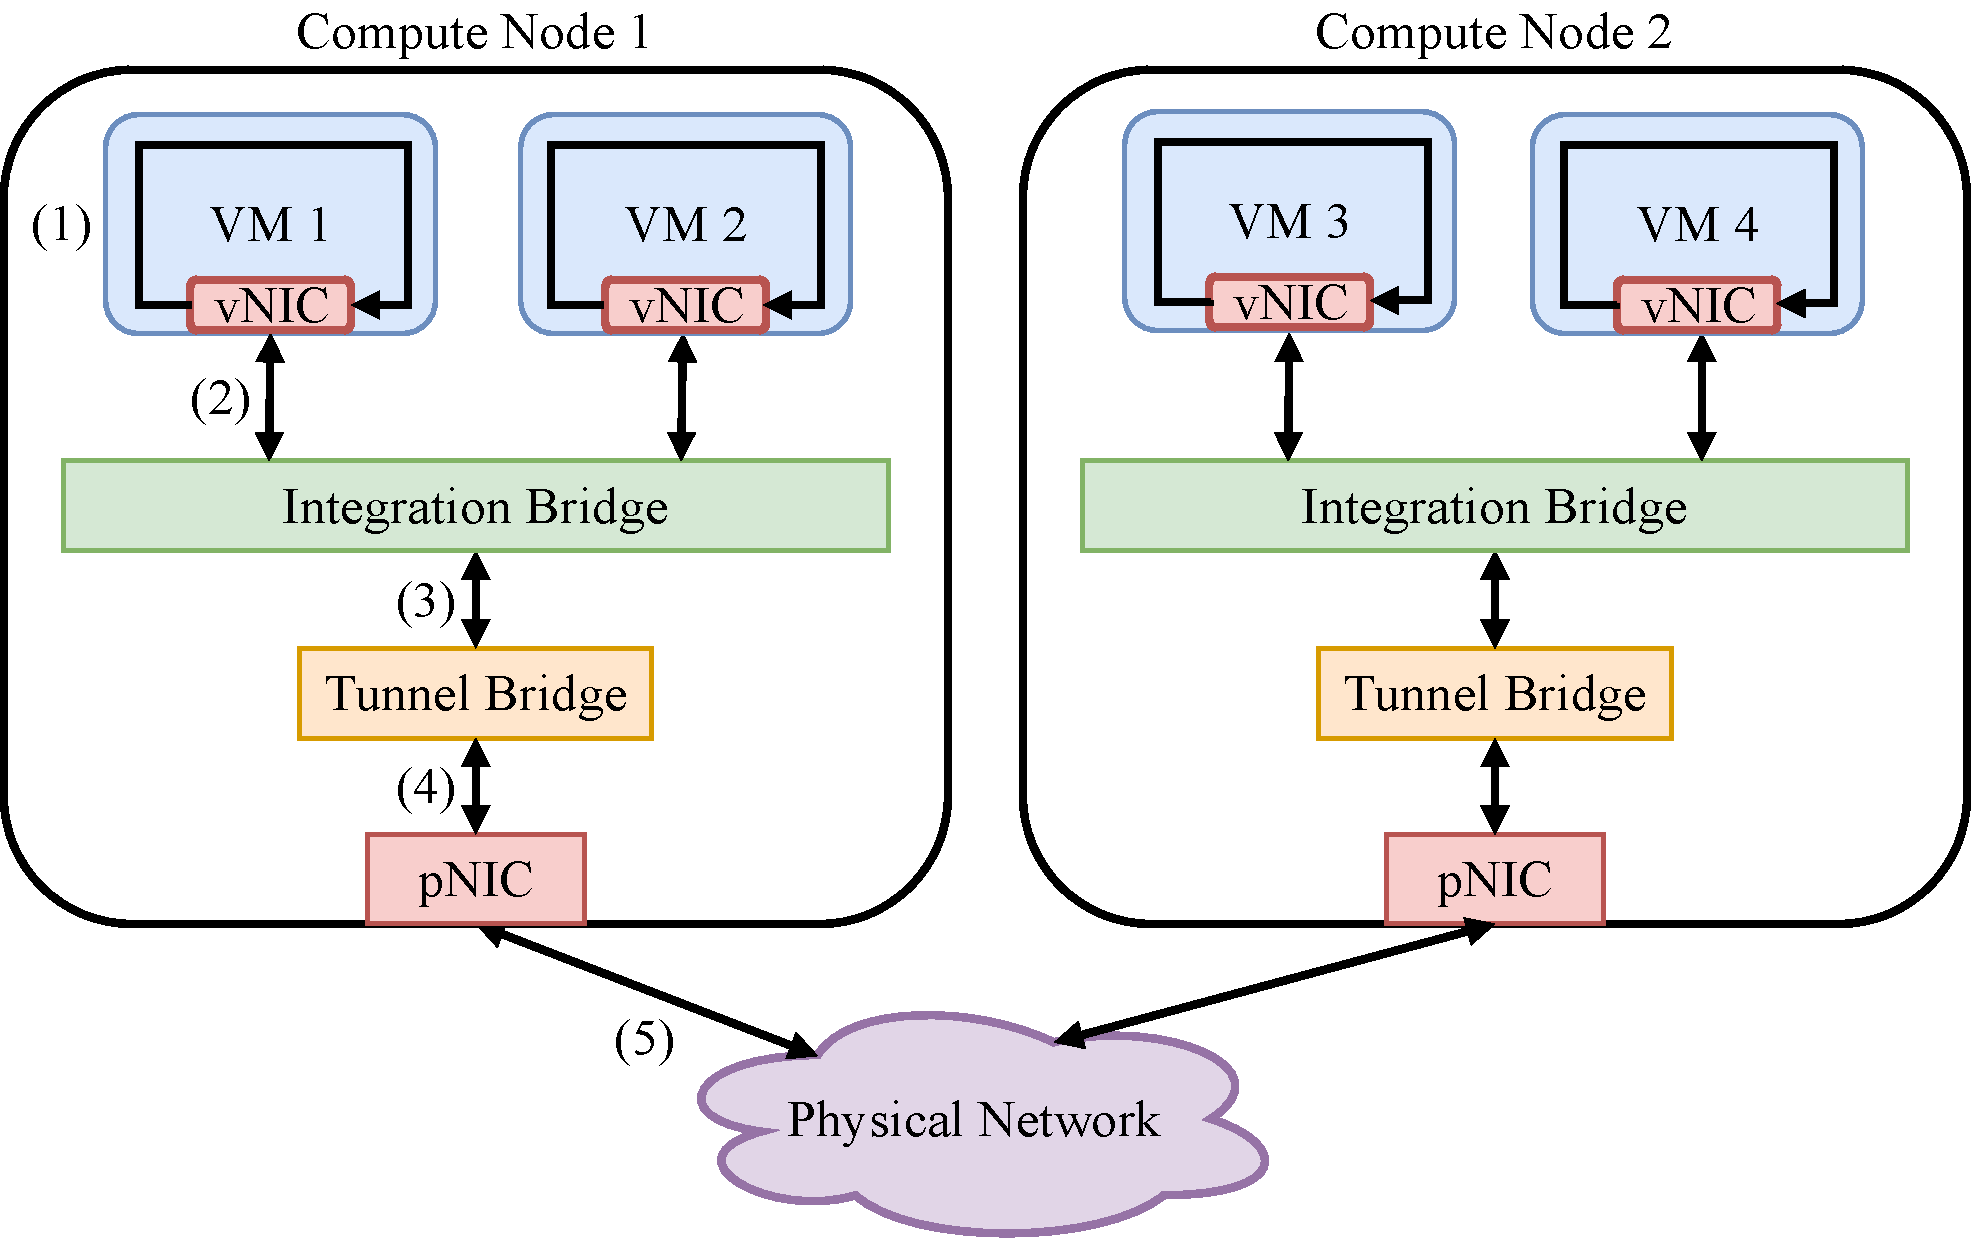
\includegraphics[width=0.8\linewidth]{./figures/nfv_infra.pdf}
    \caption{Common components of a compute node in a NFV infrastructure}
    \label{fig:nfv_infra}
\end{figure}

The Fig.\ref{fig:nfv_infra} shows components of a compute node (can be seen as a physical elementary processing unit in
a cloud environment). Multiple Virtual Instances (VIs, can be virtual machine or container, but currently VMs are still
the most deployed and default option.) can be created and connected on different compute nodes to provide services. In
order to provide a virtual network overlay on top of the underlying physical provider network, additional bridges (most
used are virtual bridge implementations e.g. Open VSwitch) are used to provided network connectivity among VIs. For
example, VI1 and VI4 can be configured in the same virtual LAN network(in the same broadcast domain) even they are
actually on different physical nodes which can be in the different physical LANs. (Or to say l3 accessible through
routers). If VI1 send a packet to VI4, the packet needs to go through all components(1-2-3-4-5-6-7-8) where additional
latencies are incurred. Since our implementation uses virtual machines, I will use VM instead of VI in following parts.

Introduction of the path and incurred latencies:

\begin{itemize}
    \item (1) and (8) - From VI to the integration bridge (br-int) and inverse:

        \textbf{This is the latency part that we have significantly reduced with proposed approach.}

        Packets are transmitted to the VM, \textbf{processed by the VM} and sent back to the br-int.
        According to some survey paper and industry reports, with the performance improvements of virtual bridges, this
        part becomes now a bottleneck in terms of latency. (In other words, processing packets in the VM costs too much
        time.) How our approach reduce the latency will be described in \ref{sec:approaches}.

    \item (2)-(3) and (6)-(7) - From virtual network overlay to physical network and inverse:

        Latency here is mainly reduced by using \textbf{OVS-DPDK}(Open vSwitch with DPDK as
        Datapath)\href{http://docs.openvswitch.org/en/latest/intro/install/dpdk/}{OVS-DPDK Homepage}.
        We have deployed OVS-DPDK on our testbed but without any modification or optimization.

    \item (4)-(5) - Physical network transmission:
        The latency here depends on the physical network technologies which are not optimized in this paper.
        All(three) physical compute nodes are connected with Gigabit Ethernet switches (in the same LAN), all layer 3
        services (DHCP, L3 routing etc.) are provided by an additional network node in the same LAN.
        Latency here is \textbf{negligible} because of good hardware, small setup, small traffic congestion.
\end{itemize}

\section{Approaches}%
\label{sec:approaches}
\blue{Names of following approaches is to be discussed.}

Before explaining different approaches, the logical service loop is illustrated in Fig \ref{fig:service_loop}.  It shows
how each packet is received by the cloud, processed by a chain of networking services (this is the concept of service
function chain), transmitted to the requested server, processed by the server and leave the cloud. The egress SFC is
mostly optional.

The ingress and egress points are endpoints or instances that are exposed to the external network (outside of the cloud
network which is commonly a dedicated private network.). For e.g. security considerations, not all internal components
are exposed to the external network. Therefore, ingress and egress points are required for clients in the external
network to have access to the cloud services. Here the components of the ingress service chain shows the common logical
function units of a service chain, namely an ordered set of virtualized network functions (VNFs). Some of these
functions can be performed parallel and some of them required to be piped and work as a pipeline.

Because the latency before the packet arriving at the ingress point and after it leaving the egress point is fully
depends on the external network setup(e.g. cable or fiber are used. it's out of scope of our optimizations). We have
measured the latency between ingress and egress points with \textbf{only one} VNF and a server in the middle. This is the RTT value
plotted in the Fig \ref{fig:service_loop_latency}. To make things simple(or independent from the service application),
the server here is just a bounce-server: receive a packet and send this packet out without doing anything. And the
VNFs in the chain perform the elementary forwarding function (Can also perform network coding, XOR and simple
encryption). Based on this loop, three approaches are explained as following.

\begin{figure}[htpb]
    \centering
    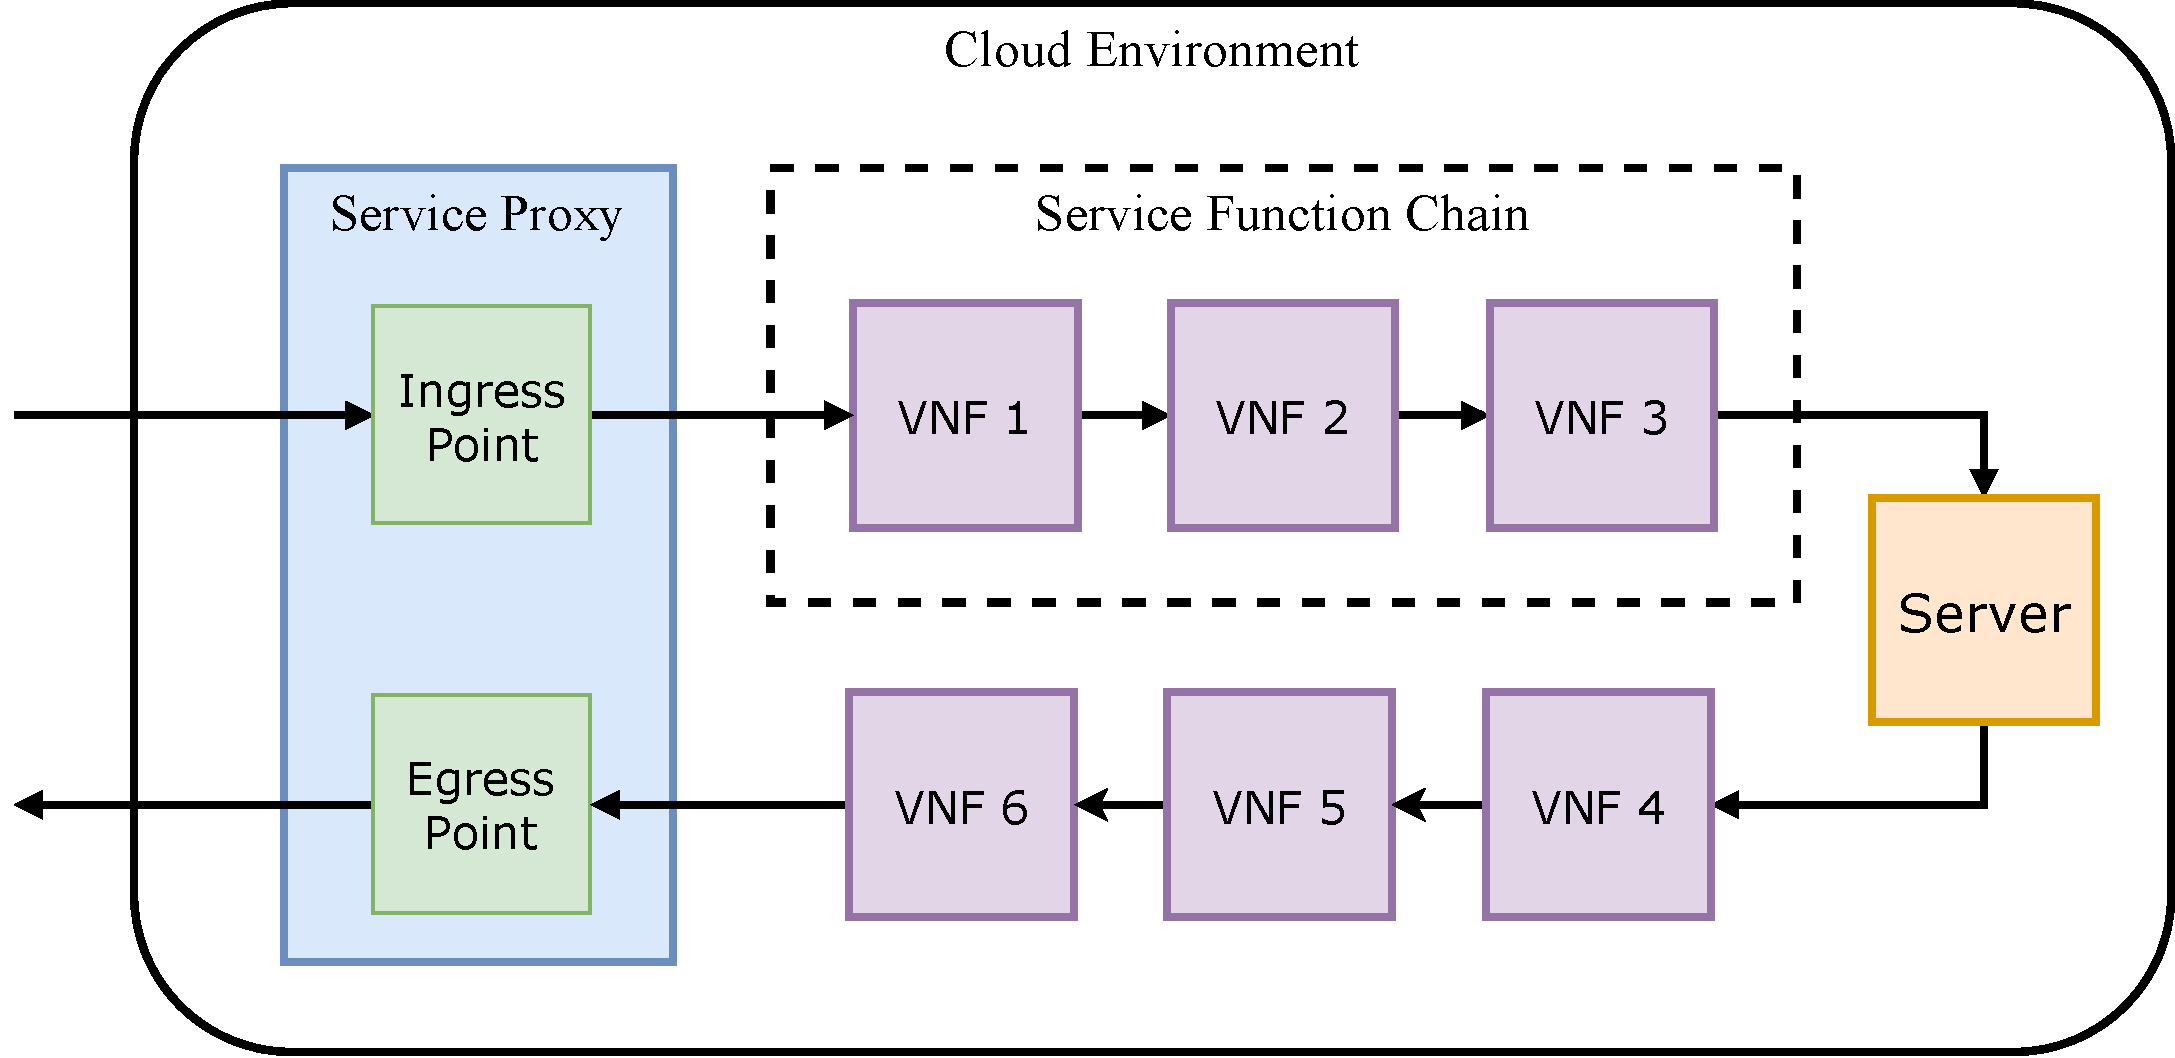
\includegraphics[width=1\linewidth]{./figures/service_path.pdf}
    \caption{Service Loop inside Cloud}
    \label{fig:service_loop}
\end{figure}

\begin{figure}[htpb]
    \centering
    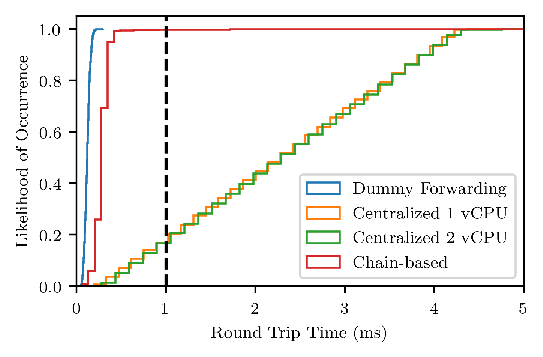
\includegraphics[width=1\linewidth]{./figures/rtt_cdf_ipd_5ms.pdf}
    \caption{Service Loop Latency}
    \label{fig:service_loop_latency}
\end{figure}

\subsubsection{Direct Connection or Dummy Forwarding}%
\label{ssub:direct_connection_or_dummy_forwarding}

As plotted in the Fig \ref{fig:service_loop}, this means directly connect(shorten) the ingress and egress points. With
this approach, the cloud does nothing on packets. This can be used as the baseline to evaluate the overhead introduced
by following approaches. This can be also used as an indicator for our basic setup. It shows that our OpenStack cluster
introduce already about 100 microseconds (us).

\subsection{Centralized Approach (Try to put all VNFs in a single VM)}%
\label{sub:centralized}

The components of the centralized approach is showed in the Fig \ref{fig:centralized_approach}.
The consideration here is to pack every VNFs in a single VM to avoid the latency introduced by transmission between VMs
(We can indicate in the related work, this latency is negligible now).

\red{In order to make multiple VNFs cooperate properly}, both kernel and user space tools need to be used. As illustrated in
the Fig, the packet needs to be transmitted between kernel space and user space at least 4 times (red lines mean slow
path or bottleneck). Additional copies of packets between kernel and user space introduce non-negligible latency
especially in a virtual guest operating system. Besides this, the resources, especially virtual CPU, need to be shared
between multiple processes both in kernel and user space. These context switching costs also time. Furthermore, the
cache behavior of the CPU can not be optimized because of this context switching. Some processing related instructions
can not be fetched and consistently stored in the CPU cache.

\begin{figure}[htpb]
    \centering
    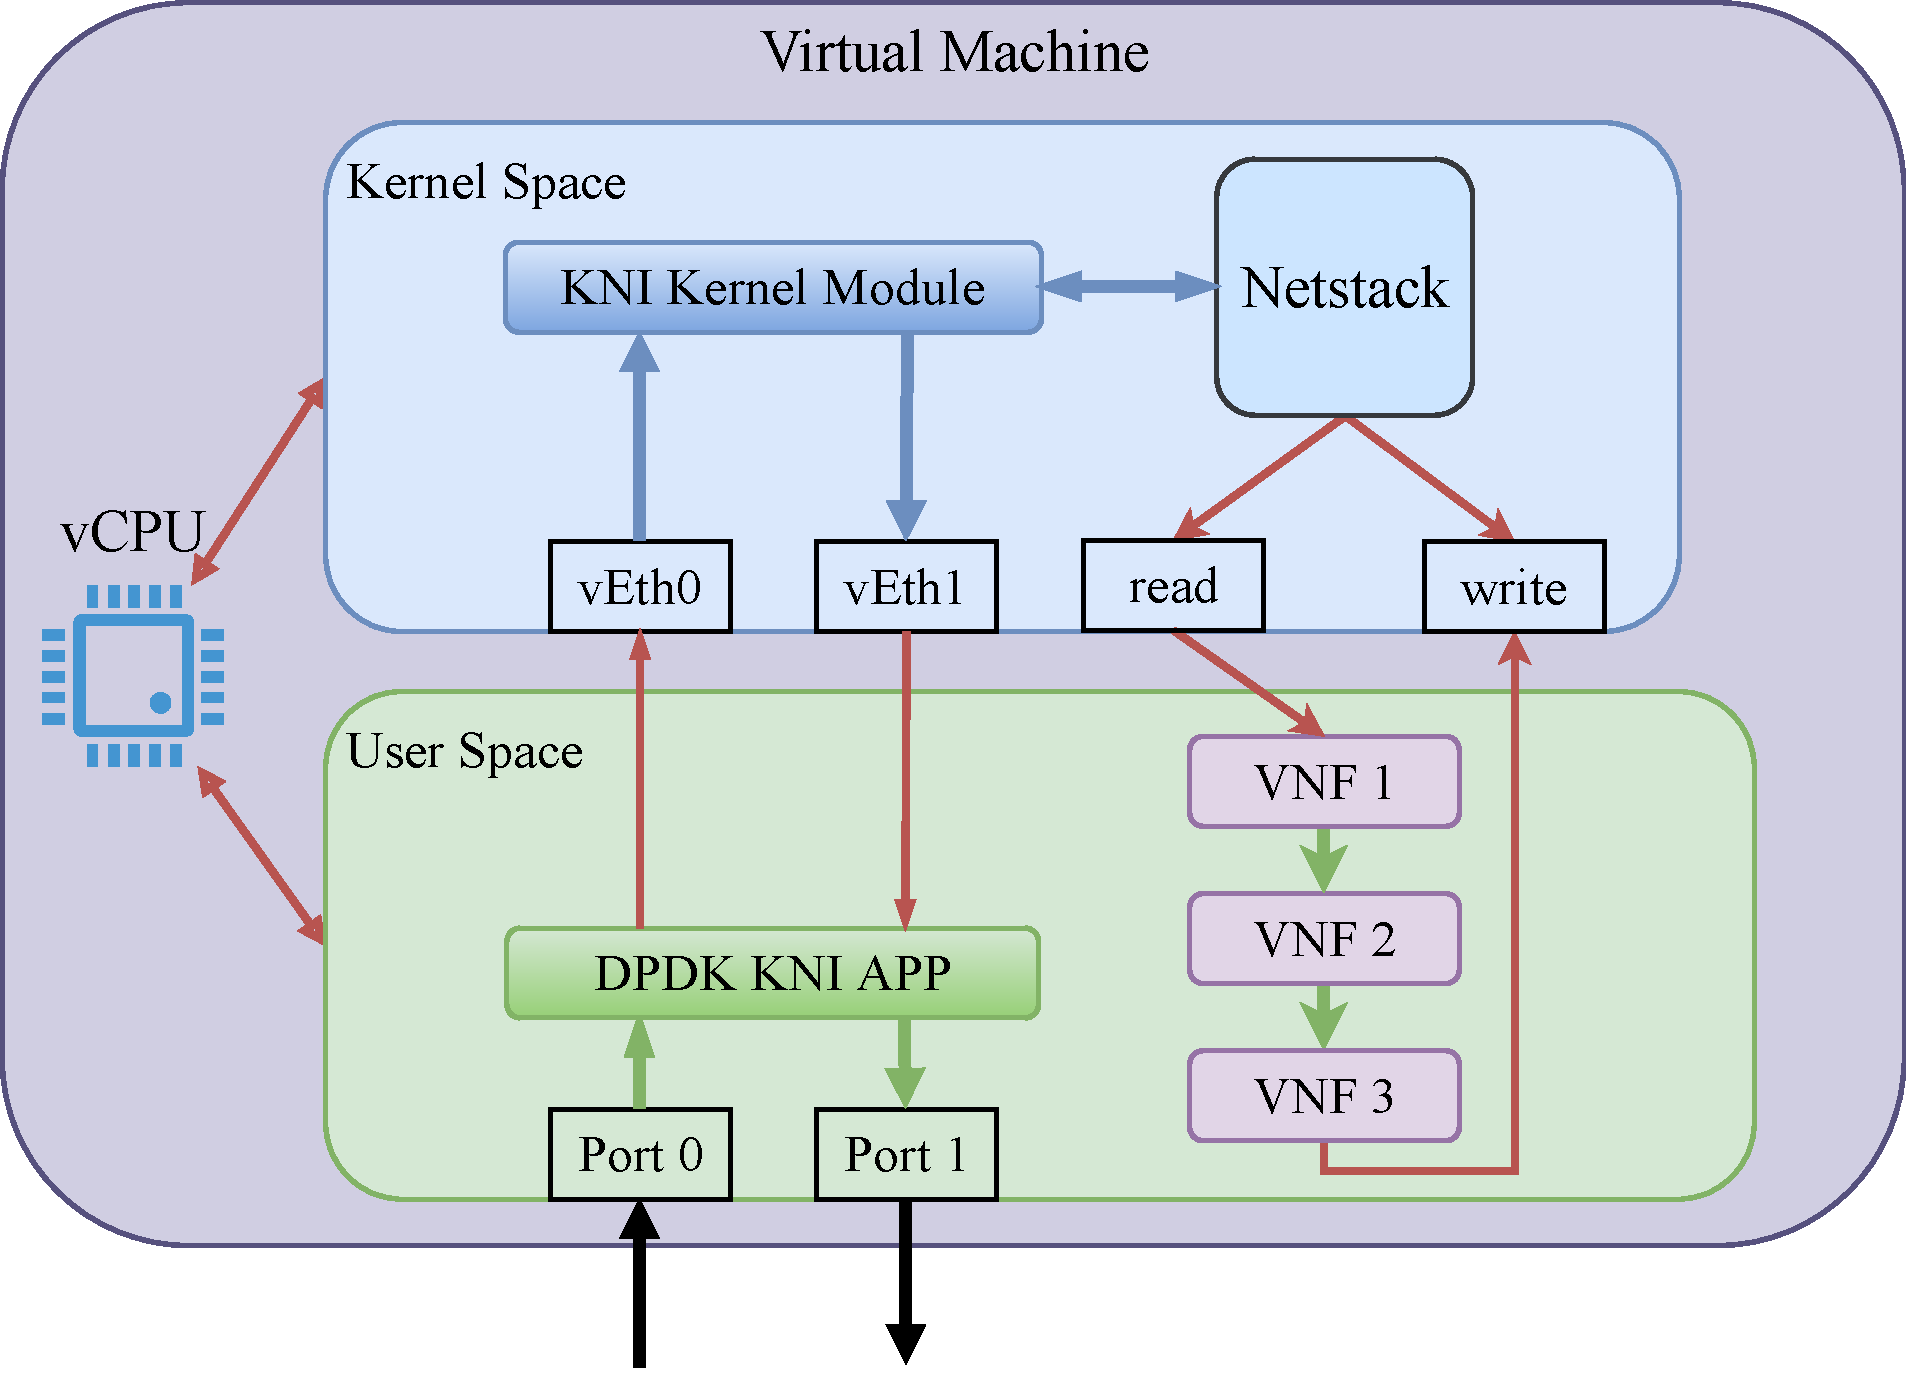
\includegraphics[width=0.7\linewidth]{./figures/centralized_approach.pdf}
    \caption{Centralized Approach}
    \label{fig:centralized_approach}
\end{figure}

\paragraph{Pros}
\begin{itemize}
    \item The VNF applications can be programmed with common socket interface, so some legacy applications can be
        deployed without modification. \red{This is the main benefit, low complexity}.
    \item Can utilize scheduler provided by the guest operating system.
    \item Can utilize features provided from kernel and user space tools at the same time.
\end{itemize}

\paragraph{Cons}
\begin{itemize}
    \item High latency.
    \item Not scalable in terms of latency. As show in the RTT results. Even if two virtual CPU are used (one core
        handle receiving packets and another core handle sending packets out), the latency can not be reduced.
    \item Not flexible for dynamically resource allocation. Since several VNFs will run the same VM, the VM should be
        provisioned with redundant resources to ensure QoS if more VNFs are added in the chain.
\end{itemize}

\subsection{Chain-Based Approach}%
\label{sub:chain_based_approach}

The in this paper proposed chain-based approach is illustrated in the Fig \ref{fig:chain_approach}.
The basic idea here is to fully separate kernel and user space for each VNF. So each VNF should run either purely in
kernel space or in the user space to avoid the latency overhead introduced by centralized approach.
So each VNF runs on a dedicated VM with its own resources. These VNFs are then connected by high-performance virtual
bridges with negligible transmission latency.

\begin{figure}[htpb]
    \centering
    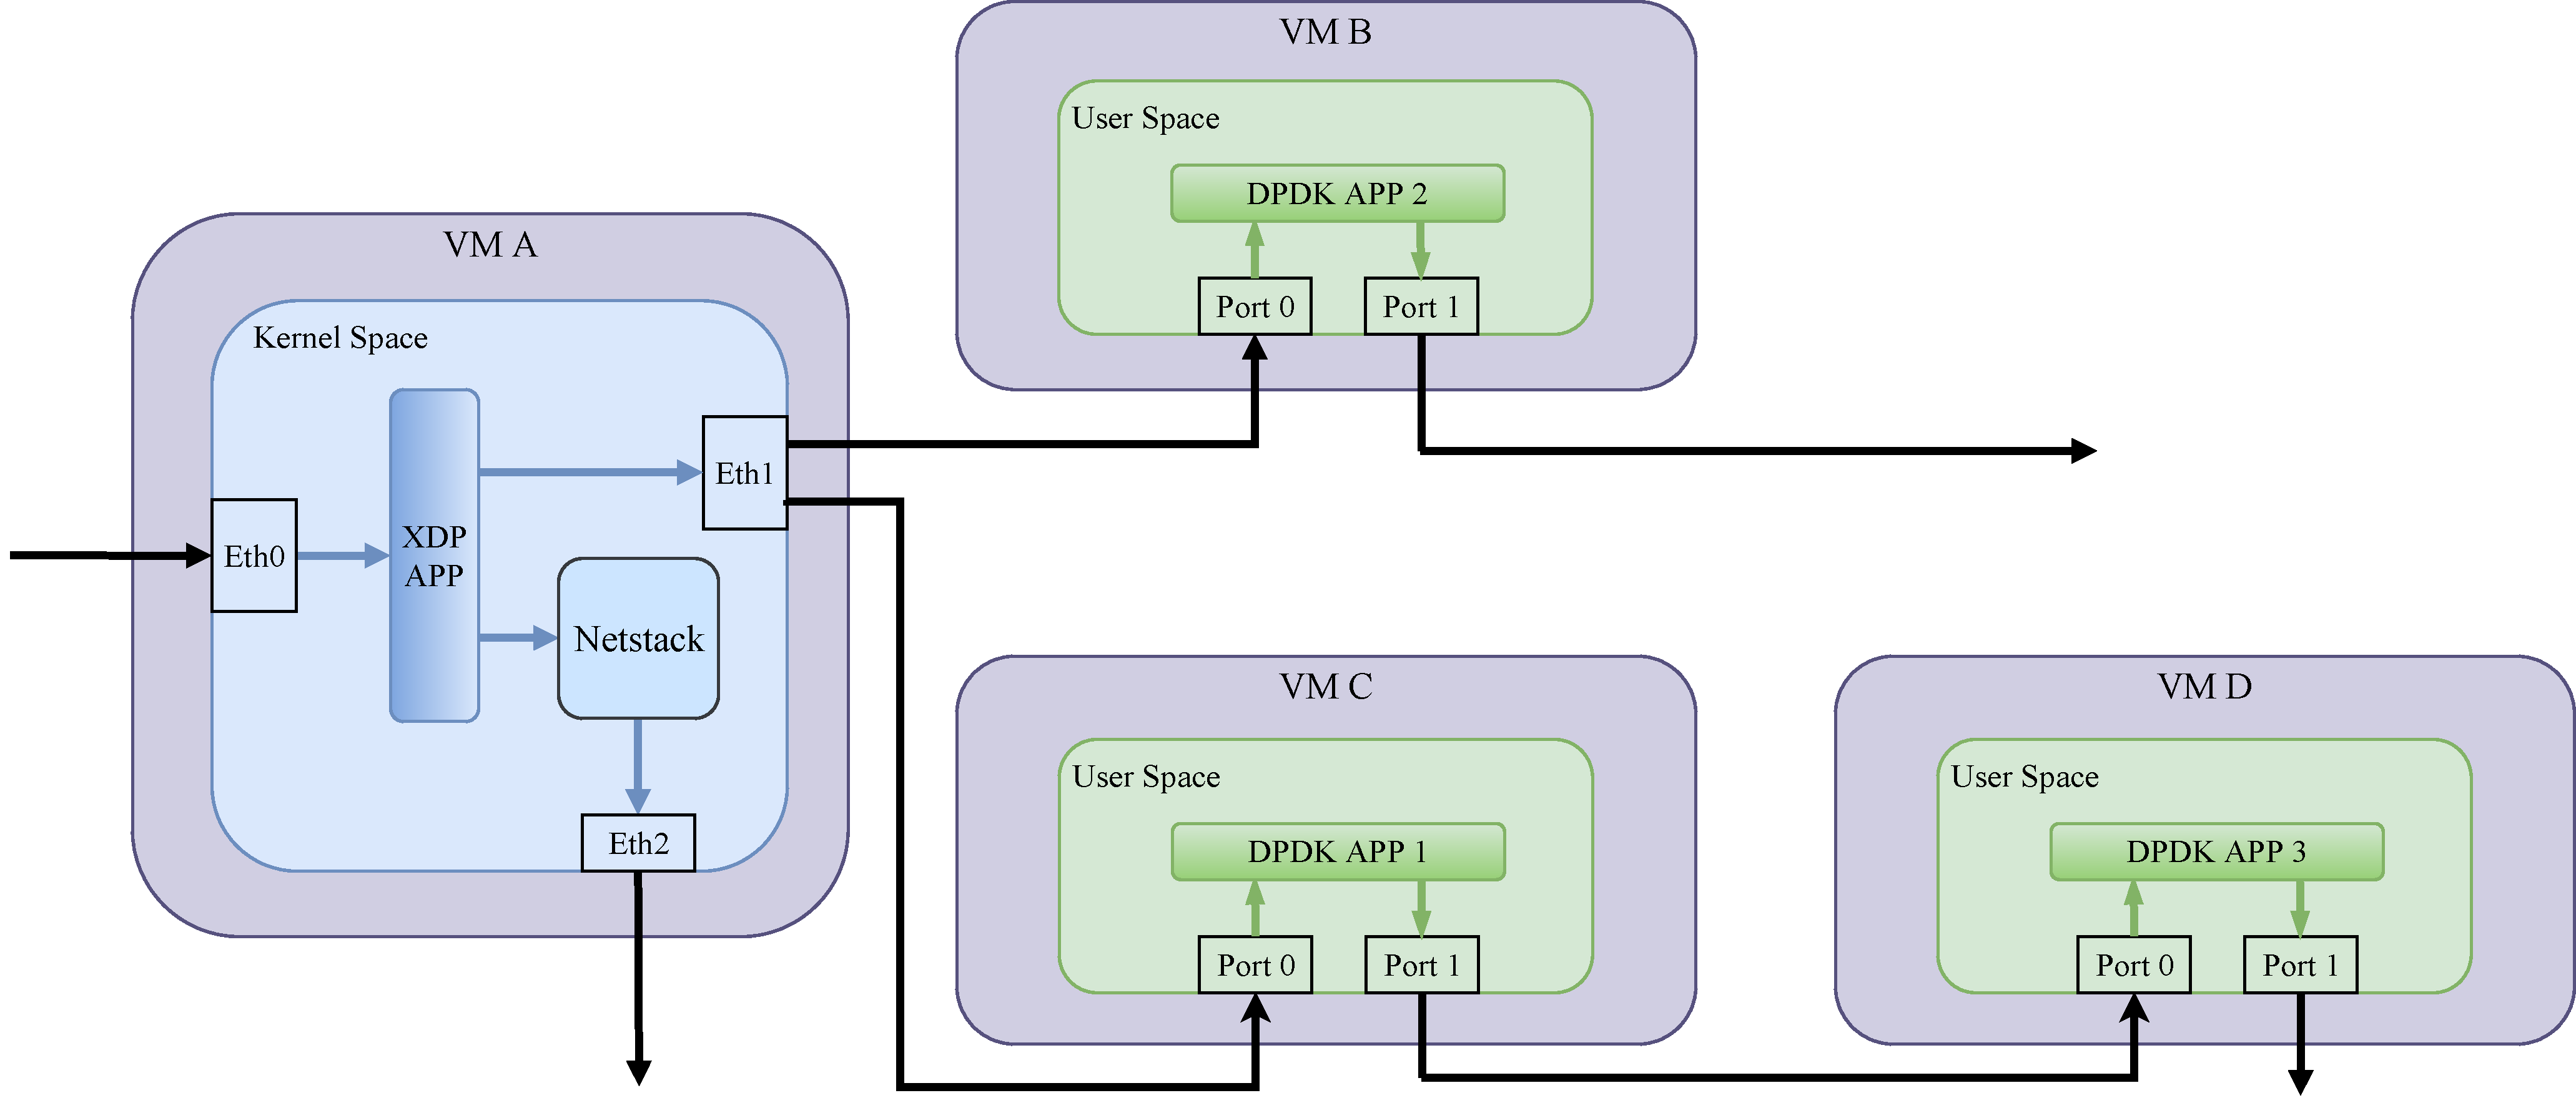
\includegraphics[width=1\linewidth]{./figures/chain_approach.pdf}
    \caption{Chain-Based Approach}
    \label{fig:chain_approach}
\end{figure}

\paragraph{Pros}
\begin{itemize}
    \item Significant reduce End-to-End latency.
    \item Flexible: New VNFs can added by extending current chain. Running VNFs can be removed or replaced dynamically.
    \item Full control of each VNF, each VNF has its own dedicated resource and runs purely in kernel or user space.
        Then each VNF can be optimized separately for its running environment for low latency without impact on other VNFs.
\end{itemize}

\paragraph{Cons}
\begin{itemize}
    \item Uses more resources. More VMs need to be created.
    \item The legacy applications need to be modified to be able to run purely in the user space.
    \item The scheduling and resource management need to be handled by the SFC orchestrator itself instead of the
        operating system.
    \item Reduce the bandwidth. Show in the Fig \ref{fig:bandwidth}. Because the application is fully optimized for low
        latency, some in kernel used strategies e.g. batching processing, are not used at all.
\end{itemize}


\begin{figure}[htpb]
    \centering
    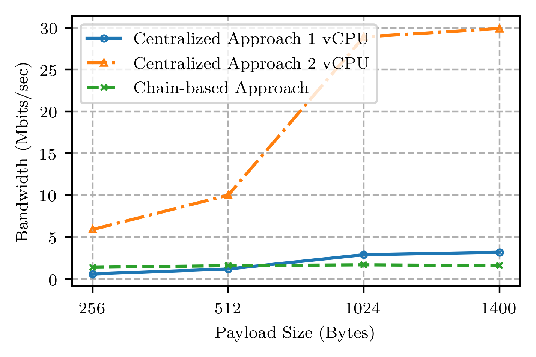
\includegraphics[width=1\linewidth]{./figures/bandwidth.pdf}
    \caption{Bandwidth comparison among approaches}
    \label{fig:bandwidth}
\end{figure}

\end{document}
